\chapter{Háttér}

A feladat egy grafikus C++ alkalmazás megvalósítása. Az alkalmazás függőségként a GLFW, GLEW könyvtárakat használja.

\section{GLFW}
A GLFW egy multiplatform ablak kezelő könyvtár. Operációs rendszertől függően implementálja az ablak megjelenítést és a bevitel kezelést. Windowson ez a Win32 API-n, Linuxon pedig a X.Org API-n keresztül történik.

\section{GLEW}
A GLEW egy multiplatform extension loader könyvtár. Ez a könyvtár dönti el, hogy operációs rendszertől és hardvertől függően melyik OpenGL extension-öket kell vagy lehet betölteni az alkalmazáshoz.

Ezeket felhasználva az alkalmazás már képes egy üres ablakot megjeleníteni és egér illetve  billentyűzet bevitelt kezelni. Tovább haladva biztosítsunk egy vizuális felületet a felhasználó számára az ImGui könyvtárral.

\section{OpenGL}

Az OpenGL \cite{OpenGL} (Open Graphics Library) egy szabvány, melyet a Silicon Graphics nevű amerikai cég fejlesztett ki 1992-ben. Segítségével egy egyszerű, szabványos felületen keresztül megvalósítható a grafikus kártya kezelése. Ezek segítségével olyan alkalmazásokat hozhatunk létre melyek képesek gyorsabb teljesítményt elérni az által, hogy nem a processzor végez minden számítási feladatot hanem egy részét kiosztja a videókártya számára. 

Széleskörűen használják számítógép által támogatott tervezésben, gyártásban (CAD/CAE), virtuális és augmentált valóság megteremtésében. Ezenkívül használják videojátékokban, Windows, Linux platformokon illettve mobiltelefonokon, konzolokon és emulátorokon is. Beágyazott rendszereken az OpenGL ES változata a legelterjedtebb.

A grafikus kártyák legnagyobb erőssége abban rejlik, hogy képesek bizonyos számítási műveleteket egyszerre párhuzamosan több adaton is elvégezni(Single data, multiple instructions SIMD). Ezek tipikusan mátrixokkal és vektorokkal kapcsolatos számítási műveletek.

A nyílt forráskódú szoftverfejlesztés közösségében kifejezetten elterjedt, hiszen az OpenGL rendelkezik a legtöbb nyíltforráskódú implementációval.

Érdemes még megemlíteni az OpenGL vetélytársait: a zárt forráskódú DirectX-et melyet a Mircosoft fejleszt és a feltörekvő szintén nyíltforráskódú Vulkan-t.

\newpage

\subsection{Az OpenGL grafikus csővezeték}
Akárhányszor egy rajzolási műveletet végzünk, ez a \ref{fig:graphics_pipeline} ábrán látható grafikus csővezetéken  keresztül történik. A grafikus csővezeték öt lépésből épül fel.

\begin{figure}[h]
    \centering
    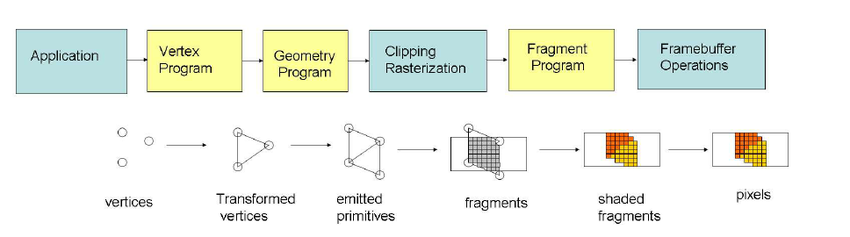
\includegraphics[width=\textwidth,height=\textheight,keepaspectratio]
    {resources/graphics_pipeline.png}
    \caption{Az OpenGL grafikus csővezeték\cite{OpenGLGraphicsPipeline}}
    \label{fig:graphics_pipeline}
\end{figure}

\subsection*{Vertex feldolgozás}
\begin{enumerate}
    \item A vertexeket egyesével beolvassuk a video memóriába, úgy nevezett VAOk-ból (Vertex Array Object), melyek a memóriában léteznek.
    \item Opcionális, primitív tesszelálása, bonyolult geometriai alakzatok felbontása egyszerűbb alakzatokká.
    \item Opcionális, primitívek feldolgozása geometria shaderrel.
\end{enumerate}

\subsection*{Vertex utófeldogolzás}
Ebben a fázisban az előző fázis kimenetén igazítunk vagy módosítunk.

\begin{enumerate}
    \item Úgynevezet transform feedback, ahol a vertex feldolgozás kimenetét buffer objektumokba mentjük. Ezáltal képesek vagyunk megőrizni a transzformáció utáni állapotot és ezt az adatot eztuán többször is felhasználni.
    \item Primitív Assembly, ahol a vertexek összekötésével valamilyen alakzatot képzünk.
    \item Primitívek fedésének feloldása, perspektíva felosztása, és a nézetablak transzformáció az ablak térbe.
\end{enumerate}

\subsection*{Raszterizáció}
A raszterizáció az a folyamat amikor egy alakzatokból álló vektor képet, pixelekből felépülő raszter képpé alakítunk. A raszterizáció az egyik leggyakoribb technika amit a számítógépes grafikában használunk, nagyon gyors folyamat ezért a grafikus motorok valós időben alkalmazzák. A raszterizáció szimplán csak annak a kiszámítása, hogy a térben lévő geometriákat hogyan alakítsuk pixelekké. A pixelek színét pedig a fragmens shader határozza meg.

\subsection*{Fragmens shader}
A programozható fragmens shader ami minden fragmenst feldolgoz és már a monitoron megjeleníthető kimenetet készít.

\subsection*{Mintánkénti feldolgozás}
\begin{enumerate}
    \item Scissor teszt, ami levágja azokat a fragmenseket amik nem férnek bele a megjelenítendő képbe.
    \item Stencil teszt, ahol a stencil bufferben tárolt értékek alapján elhagyhatunk fragmenseket.
    \item Depth teszt, mélység érzet keltése, minél távolabb van egy fragmens a térben, annál világosabb lesz a színe.
    \item Blending teszt, ezáltal érhető el az átlátszóság vagy az üveg hatás keltése, alpha érték alpaján az egymást fedő pixelek színe keveredik.
    \item Logikai műveletek, melyeket a fragmens színeit ábrázoló biteken végezhetünk.
    \item Write mask, az előző lépések használni kívánt kimeneteit egy maszkban egyesíti.
\end{enumerate}

A grafikus pipeline-nak biztosítsuk az adatokat amiket a felhasználói felületen keresztül adhatunk meg. Ezek az adatok legyenek a következőek: vertexenként kilenc darab float érték, ebből az első három darab a vertex kordináták, második három darab a szín értékek, a harmadik három darab pedig a textúra kordináták. Kelleni fog még indexenként egy unsigned integer, a vertex és fragmens programok forráskódja, illetve a használni kívánt textúrák elérési útja.

A rendereléshez minden szükséges adat megvan a textúra adatokon kívül, ezekhez jelenleg csak az elérési útvonalak vannak meg. Az útvonalon keresztül olvassuk be a kép adatokat az stb\_image könyvtár segítsével.

\section{Dear ImGui}
Az ImGui egy úgynevezett "Immediate mode graphical user interface", azaz jellemzően a felhasználói felület ugyanazon a szálon fut mint az alkalmazás, hogy a lokális adatokat is elérje. Függvény hívásokból épül fel ahelyett, hogy a UI felépítése valamilyen leíró nyelven lenne egy külön fájlban meghatározva. Leggyakoribban grafikus alkalmazások debugolására használják mert használata nagyon egyszerű, gyors, intuitív és nem különösebben befolyásolja az alkalmazás teljesítményét. A kinézet testreszabása terén viszont nem ad túl nagy szabadságot a fejlesztő számára.

Ezen a ponton van már egy felhasználói felületünk amin keresztül meg tudunk hívni függvényeket,képesek vagyunk változtatni változók értékén. Most már elkezdhetjük a grafikát implementálni az OpenGL segítségével.

\section{Kép összehasonlítás}
Most már minden adatunk megvan egy kívánt kép generálásához. Két kép összehasonlítására használjuk az SSIM és Chi square distance statisztikai módszereket alkalmazó algoritmusokat. Fontos, hogy a két összehasonlítandó kép azonos felbontású legyen, különben ezek a módszerek nem alkalmasak. Utolsó lépésként ezek eredményét jelenítsük meg a felhasználó számára.

A chi square distance algoritmus\cite{CSQD} veszi két kép hisztogramját és egyesével összegzi színcsatornánként a rajzolt és a cél kép színértékeinek különbségének a négyzetét majd eloszjta a rajzolt kép színértékével. Minnél kissebb az összeg, annál jobb az egyezés. 

Az SSIM elődjét Universal quality Index (UQI)-mal hívták, melyet Zhou Wang és Alan Bovik fejlesztett ki 2001-ben. Ezt fejlesztették tovább Hamid Sheikh és Eero Simoncell segítségével azzá, amit ma SSIM-ként ismerünk\cite{SSIM}. Az SSIM algoritmust általában arra használják, hogy megvizsgálják mekkora a képromlás az eredeti kép és egy tömörített kép között. A képfeldolgozó közössében az egyik legtöbbet használt algoritmus, a Google scholar szerint a 2004-es tanulmányt több mint húszezren hivatkoztak rá azóta.

Itt is fontos, hogy a két képünk, ezek legyenek x és y képek, azonos felbontásúak legyenek, ugyanúgy mint a chi square distance esetén. Az SSIM minőségi indexet az alábbi képlet alapján kapjuk meg, melyet szintén minden csatornára ki kell számolnunk, majd összegeznünk.

\section{A GLSL shading nyelv}
Az OpenGL shading nyelv egy magas szintű shader nyelv aminek a szintaxisa leginkább a C programozási nyelvére hasonlít. Azzal a céllal készült, hogy a fejlesztőknek több irányítása legyen a grafikus csővezeték felett anélkúl, hogy shader assembly kódot kellene írniuk vagy más egyéb hardver specifikus nyelvet használni. Mint a legtöbb programozási nyelvben a program belépési pontja a main függvény. A nyelv szintén tartalmaz vektor és mátrix típusokat is, hogy a velük kapcsolatos műveletek egyszerűbbek legyenek. A programozó munkáját továbbá könnyebbítik egyéb beépített matematikai függvények mint például trigonometrikus függvények, gyökvonás, hatványozás.

\section{Elvárások az alkalmazással szemben}

\begin{itemize}
    \item Clear color azaz a háttérszín állítása
    \item Konzol amin keresztül az alkalamzás információkat oszt meg a felhasználoval szöveges formában
    \item Konzolon keresztüli alkalmazás vezérlés szöveges parancsokkal
    \item Konzolon megjelenített szövegek törlése
    \item Kódszerkesztő widget, ahol a shader forráskódokat szerkeszthetjük
    \item Fájl böngésző widget, amin keresztül fájlok elérési útjait választhatjuk ki
    \item Scene szerkesztő widget, ahol a megjelenített objektumok adatatit szerkeszthetjük
    \item Alkalmazás aktuális állapotának exportálása JSON fájlba
    \item Alkalmazás állapotának betöltése JSON fájlból
    \item Multiplatform, képes Windows és Linux operációs  rendszereken is futni
    \item Alacsony gépigény
    \item Reszponzivitás, az alkalmazást kényelmes használni
\end{itemize}

